% Score z=-1+x1+0.8*x2. Classification predicts 1 above each threshold boundary.
% Native PGFPlots; reproduced by examples/generate_foundation_figures.py.
% Constructed observations / analytical teaching example, not empirical data.
\begingroup
\definecolor{blueplot}{HTML}{4E79A7}
\definecolor{redplot}{HTML}{D95F59}
\definecolor{inkplot}{HTML}{111111}
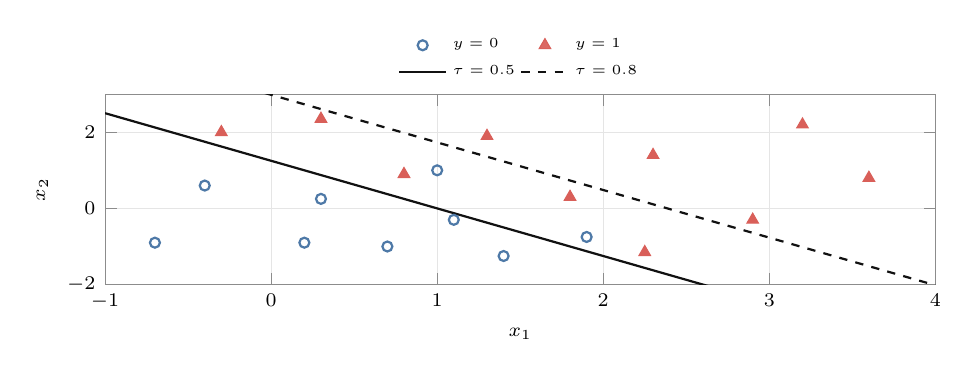
\begin{tikzpicture}
\begin{axis}[
width=\linewidth,height=4.0cm,font=\scriptsize,
tick label style={font=\scriptsize},label style={font=\scriptsize},
axis line style={black!45},tick style={black!45},
grid=major,grid style={black!10},scaled ticks=false,
clip=true,unbounded coords=jump,
legend style={font=\tiny,draw=none,fill=white,fill opacity=.94,text opacity=1,
  legend cell align=left,inner sep=2pt,row sep=1pt},
xmin=-1,xmax=4,ymin=-2,ymax=3,
xlabel={$x_1$},ylabel={$x_2$},xtick={-1,0,1,2,3,4},ytick={-2,0,2},
legend style={at={(.5,1.02)},anchor=south},legend columns=2
]
\addplot[blueplot,only marks,mark=o,thick,mark size=1.8pt] coordinates {(-0.7,-0.9) (-0.4,0.6) (0.2,-0.9) (0.3,0.25) (0.7,-1) (1.1,-0.3) (1.4,-1.25) (1.9,-0.75) (1,1)};
\addlegendentry{$y=0$}
\addplot[redplot,only marks,mark=triangle*,mark size=2.4pt] coordinates {(-0.3,2) (0.3,2.35) (0.8,0.9) (1.3,1.9) (1.8,0.3) (2.3,1.4) (2.9,-0.3) (3.2,2.2) (3.6,0.8) (2.25,-1.15)};
\addlegendentry{$y=1$}
\addplot[inkplot,thick,no marks] coordinates {(-1,2.5) (4,-3.75)};
\addlegendentry{$\tau=0.5$}
\addplot[inkplot,thick,dashed,no marks] coordinates {(-1,4.232867951) (4,-2.017132049)};
\addlegendentry{$\tau=0.8$}

\end{axis}
\end{tikzpicture}
\endgroup
